\Chapter{SYNTHETIC DATA GENERATION}\label{sec:Syn}


The framework of this study relies on synthetic data. The performance signature vectors are based on synthetic data generated from each model of the performance space.  Therefore, we dedicate a full chapter to the process of generating synthetic data from the different models.

A unique advantage of synthetic data is that the model parameters can be predefined. Once the simulated data is generated with predefined parameters, a model can be trained over the generated data and a comparison with the original, known parameter values becomes possible. This may be the strongest benefit of synthetic data in assessing model fit. Since the hypothesis of this research relies on comparison the performance vector of real vs. synthetic data, then we can also consider data specific parameters of the real data in the generation process to make a better comparison of the results.

\section{Data generation parameters}
%(2) explain how they are either derived from data, or initialized (presumably from a random distribution); 
As described before, there exists two types of parameters for student test outcome:
\begin{itemize}
\item Model specific: Models have their own parameters, some of which may be shared among models, such as a Q-matrix for multiple skills models, some of which are more unique such as the item discrimination parameter of the IRT class of models. Generally an experiment should be designed to learn these parameters form a dataset or they can be generated under specific criteria. More details for each parameter is given later in this chapter.
\item Data specific (contextual): The data specific parameters are common to all data sets.  They have to be predefined, but they may be set to reflect a data set for which we want to find the ground thruth.  For example, the item difficulty distribution or the student success rate distribution are two data specific parameters.  Data specific parameters can also be a model parameter, such as item difficulty and discrimination.
\end{itemize}

Table \ref{tbl:param-DataGen} shows a complete list of both types of parameters required for data generation.

%\newcommand{\tabitem}{~~\llap{\textbullet}~~}
%\newcommand\VRule[1][\arrayrulewidth]{\vrule width #1}

\begin{table}
  \centering

\begin{tabular}{c|c|l!{\VRule[1.5pt]}l|l!{\VRule[1.5pt]}l|}
\multicolumn{3}{c}{}&\multicolumn{3}{c}{Parameters}\tabularnewline
\cline{4-6}
\multicolumn{3}{c!{\VRule[1.5pt]}}{Skills Model}&\multicolumn{2}{c!{\VRule[1.5pt]}}{Model specific}&\multicolumn{1}{c|}{Data specific}\tabularnewline
\cmidrule[1.5pt]{2-6}
&&NMF Conj. & & &  \tabularnewline
\cline{3-3}
&&NMF Add.&&\multirow{-2}{*}{ \tabitem  Q-matrix }&\multirow{-2}{*}{\tabitem Number of students } \tabularnewline
\cline{3-4}
&&DINA& \tabitem Slip & &\tabularnewline
\cline{3-3} 
&\multirow{-4}{*}{\begin{sideways} \scriptsize Multiple\end{sideways}}&DINO& \tabitem Guess&\multirow{-2}{*}{  \parbox[t]{3cm}{ \tabitem Students skills  \\ mastery matrix}}& \multirow{-2}{*}{\tabitem Number of items } \tabularnewline
\cmidrule[1.5pt]{2-5}
&&&\multicolumn{2}{l!{\VRule[1.5pt]}}{\tabitem Student ability  } &  \tabularnewline
&&&\multicolumn{2}{l!{\VRule[1.5pt]}}{\tabitem Item difficulty  } &\multirow{-2}{*}{\tabitem Number of skills } \tabularnewline
&&\multirow{-3}{*}{ IRT}&\multicolumn{2}{l!{\VRule[1.5pt]}}{\tabitem Item discrimination}  &\tabularnewline
\cline{3-5}
&&&\multicolumn{2}{l!{\VRule[1.5pt]}}{\tabitem Student Odds  } & \multirow{-2}{*}{\tabitem Test success rate }  \tabularnewline
&\multirow{-5}{*}{\begin{sideways} \scriptsize Single \end{sideways}}&\multirow{-2}{*}{ Expected}&\multicolumn{2}{l!{\VRule[1.5pt]}}{\tabitem Item Odds}  &  \tabularnewline
\cmidrule[1.5pt]{2-5}
&&&\multicolumn{2}{l!{\VRule[1.5pt]}}{\tabitem Initial Odds } & \multirow{-2}{*}{\tabitem Student score Variance} \tabularnewline
&&&\multicolumn{2}{l!{\VRule[1.5pt]}}{ \tabitem Odds ratio } & \tabularnewline
\multirow{-9}{*}{\begin{sideways} \scriptsize Contributed skills \end{sideways}}&\multirow{-3}{*}{\begin{sideways} \scriptsize Zero\end{sideways}}&\multirow{-3}{*}{ POKS }&\multicolumn{2}{l!{\VRule[1.5pt]}}{\tabitem \parbox[t]{.4\textwidth}{\raggedright Partial Order Knowledge Structure (KS) (includes two alpha error parameters for its induction from data)}}& \multirow{-2}{*}{\tabitem Item score Variance} \tabularnewline
\cmidrule[1.5pt]{2-6}
\end{tabular}
  \caption{Parameters involved in synthetic data generation}
  \label{tbl:param-DataGen}
  \note{Item difficulty and other ``model specific'' parameter can be obtained from data.  We may have to refine this taxonomy, but let's leave it as is for now.}
\end{table}

\subsection{Assessing parameters}

To generate synthetic data, a model and data specific parameters are required There are two approaches to obtain these parameters to generate synthetic data:
\begin{itemize}
\item Parameters estimated form real data: In general, models define means to estimate their parameters from data.  Some are trivial to estimate, such as student success rate distribution if we assume a Gaussian distribution, for eg., and some are much more complex, which is the case of latent factors such as the number of skills and the Q-matrix itself.
\item Parameters generated randomly based on a distribution: In the case that there exists no reference dataset to derive parameters we can randomly select some samples based on a distribution (for example normal distribution). Some parameters have specific conditions that if they become violated it changes the definition of the parameter. More details is given in next sections.
\par\note{This isn't quite right I think.  We can estimate the distribution parameters from the data and still generate random parameter distributions.}
\item Expert given and arbitrary parameters: Latent factors are often not derived from data but arbitrarily defined by expert or by some educated choice.  The Q-matrix is the most obvious of such parameter, but so are the guess and slip parameters which can prove difficult to correctly estimate from data.

\end{itemize}


The rest of this chapter describes the data generation process based on each model assessment technique that is used in the proposed model selection approach.
% we can also specify which paramters has been borrowed from real data and which one has been generated

\section{POKS}
POKS is a technique that categorized as a ``zero skills'' method which does not directly attempt to model underlying skills but instead rely on observable items only. 

\subsection{Obtaining parameters}
This model has three parameters with which the inference in possible: Knowledge structure, Initial probabilities, Odds ratio. To extract these parameters from an existing data we use POKS \footnote{http://www.professeurs.polymtl.ca/michel.desmarais/Papers/UMAP2011/lib-poks.R} R package to learn all the parameters given a dataset. In the case that the data in not available these parameters should be generated randomly. Below we will describe how these parameters are generated with different conditions and constraints.
%\note{Suggestion: (1) formally define all the parameters of the simulation,
\subsubsection{Partial Order Knowledge Structure (KS)}
This parameter shows the relation and the dependency among a set of items. In fact, it reflects the order of learning a set of items in the same problem domain. Assuming items as different ``nodes'' in the graphical structure, there is a kind of ``parent-child'' relation between some pair of nodes where an easier item can be the child of a harder item. In our study this relation is considered as a ``link'' between two nodes. This link is not necessarily exists between each pair. Only those items that show a relation in the learning process can have a pairwise link. 

A knowledge structure is a directed acyclic graph, with the exception that cycles in the form of symmetric relations are allowed. Also in the current version of POKS transitive relations between items are explicitly ignored. % because there is a likely strong correlation from transitive to direct relations that would need to be taken into account.

% if you don't have transitive relation in your process you need to state that please


There are two other parameters involved in the generation of KS:
\begin{itemize}
\item Conditional probability strength.  For a link to be established between two items, say $X_a \rightarrow X_b$, the data must reveal a minimal conditional probability greater than a threshold $\alpha_p$: $P(X_b|X_a) > \alpha_p$.
% Number of independent graphs: Even in a set of items there could be different groups of nodes without any dependency between each group. Since there is no link between each group then they create an in dependent graph in the knowledge structure. This parameter can also affect the total number of links in a structure where more independent groups results in less number of links in the structure given same density of links in each group. 
\item %Interaction test.  Moreover, the conditional probability must be different than the unconditional probability: $P(X_b|X_a) \neq P(X_b)$.  This is tested with an interaction test such as the $\chi^2$ test using a given alpha error, $\alpha_c$.
Total Number of links: This has a correlation with the previous parameter but still we can control the number of dependencies in a KS. This parameter has a direct effect on test success rate and item score variance. Fewer number of links will result in lower test success rate and item score variance.% There are still some other parameters that could change the test success rate and item score variance.
\end{itemize}
%In the current study, the two parameters, $\alpha_p$ and $\alpha_c$, are respectively set at~$0.5$ and~$0.2$. \note{verify this}
Other input parameters can make the random generation more specific,such as the number of links and number of independent trees in a KS\note{?? Needs to be defined.}. These parameters will change the item variance in the test result matrix. 

\begin{figure}[t]
\centering 
\subfigure[Adjacency matrix ]{  $\begin{array}{ccc}
&\begin{array}{ccccc}
i_{1} & i_{2} & i_{3} & i_{4}& i_{5}\end{array}&\\
\begin{array}{c}
i_{1}\\
i_{2}\\
i_{3}\\
i_{4}\\
i_{5}
\end{array}&\left[\begin{array}{ccccc}
0 & 0 & 0 & 0 &1\\
0 & 0 & 1 & 0 &0\\
0 & 0 & 0 & 1 &1\\
0 & 0 & 0 & 0 &0\\
0 & 0 & 0 & 0 &0
\end{array}\right]&\\
&&\\
&&
\end{array}$}
\qquad
\qquad
\subfigure[Graphical representation ]{ $\begin{array}{cc}
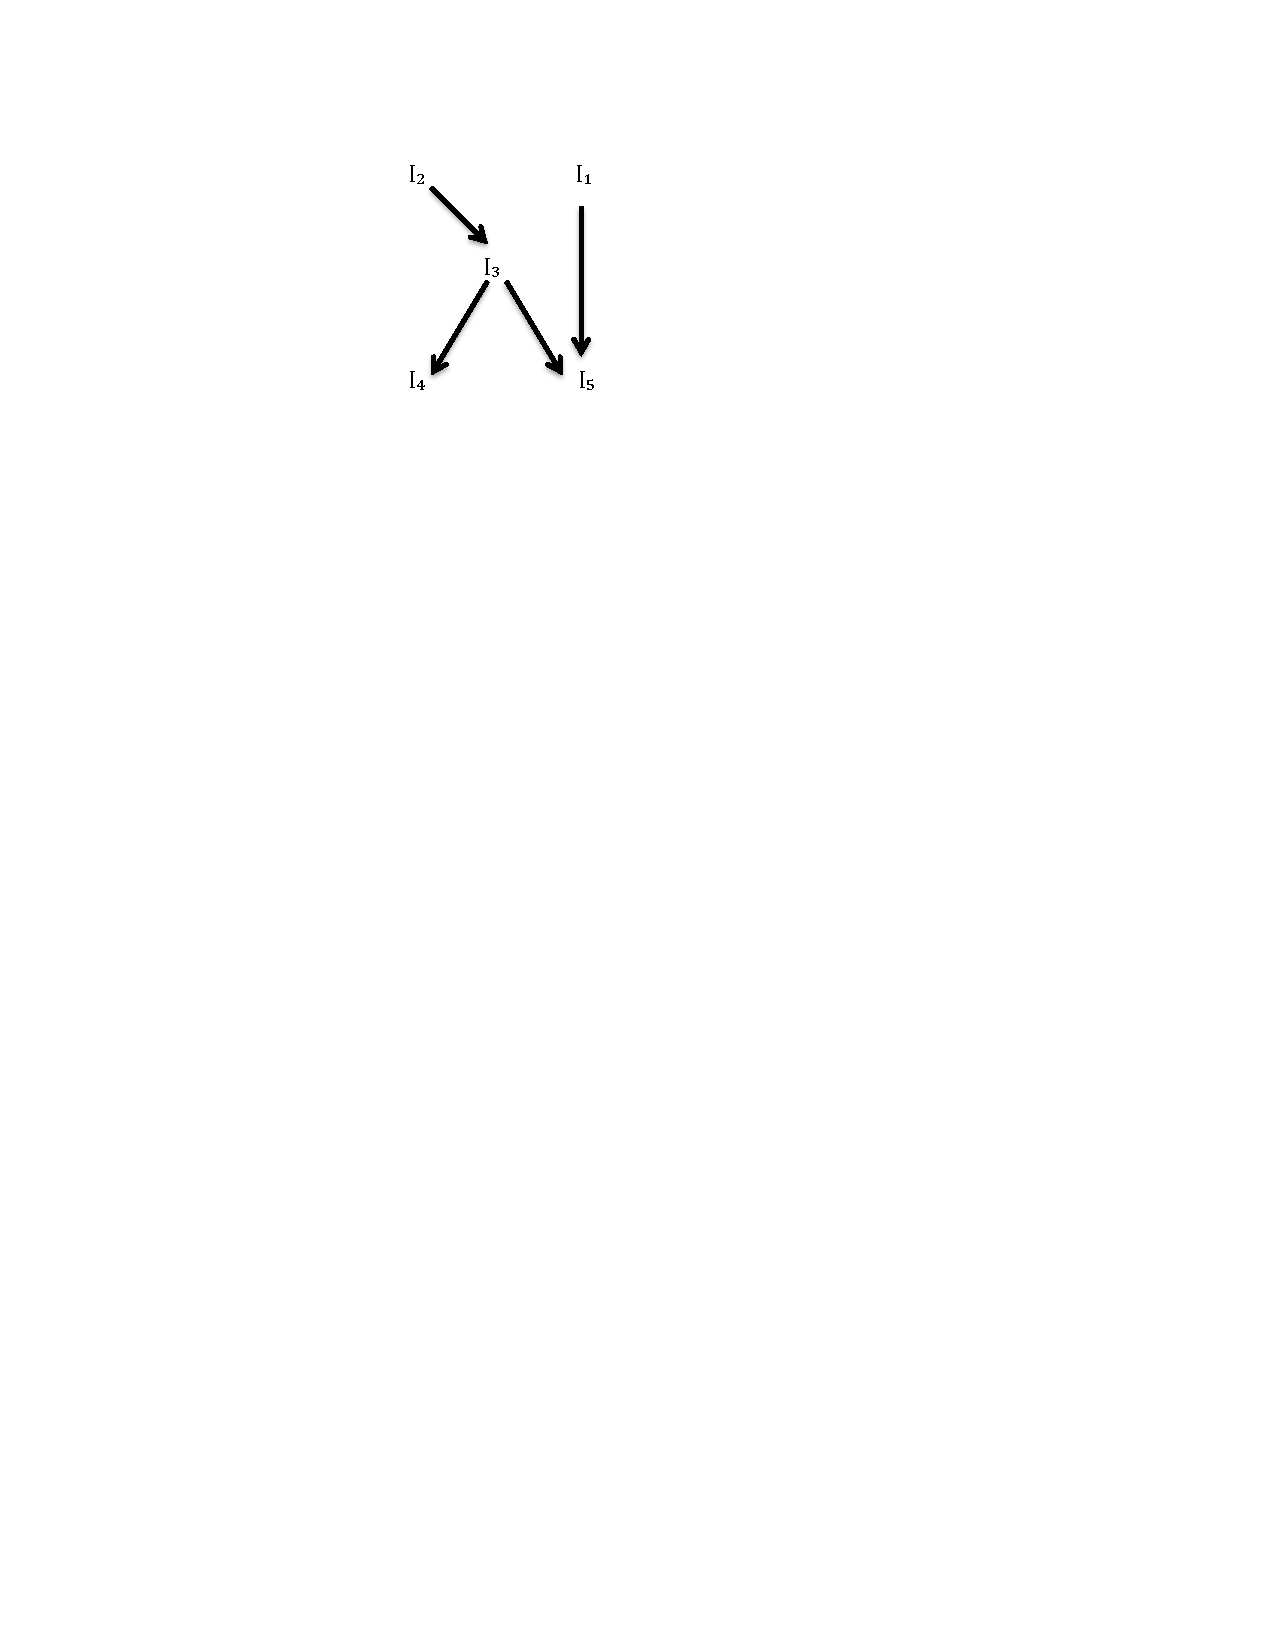
\includegraphics[trim=7cm 20.4cm 11cm 3.5cm,width=.20\linewidth]{SampleKS} &
\end{array}$}

\caption{An example of random KS with 5 items}
\label{fig:KSExample}
\end{figure}

Adjacency matrix  is one way to represent the KS. To avoid having a cycle in the structure we randomly assign $0$-$1$ values to an upper triangular of this matrix. For simplicity we consider the structure to be a single connected graph and the number of links corresponds to half of the cells of the upper triangular of this matrix. figure \ref{fig:KSExample} shows a adjacency matrix associated with its graphical structure. 

Once the KS is generated we should assign proper value to each item as an initial value and also each pair of items should be associated with an odds ratio. One of the important concepts in assigning values to initial probabilities and odds ratio (explanation is in the next subsection) is the ``level'' of a node in the graphical representation of the KS which corresponds to the longest path from that node to a leaf node. A leaf node is a node that does not have any child and a root is a node without any parents. Equation \ref{EQ:Level} shows the definition of this function where $length-of$ returns the length of a path between two nodes; and $path$ returns true value if there exists a directed path between two nodes; and $leaf$ returns true if the node is a leaf.  For example in figure \ref{fig:KSExample} $I_{5}$ is a leaf with the level of $1$ and $I_{2}$ is a root with level of $3$.

\begin{equation}
L(KS,N_{i}) = max(E|E=length-of(N_{i},p)  ,  \exists path(N_{i},p)  , leaf(p)=True)
\label{EQ:Level}
\end{equation}


%The generation of a random KS consists in randomly assigning 0-1 values to an upper triangular adjacency matrix. \annote{Once the KS adjacency matrix is created, we can assign values to each item that contributes with the initial odds of each node and odds ratio between a pair of nodes.}{not clear; odds ratio has not yet been introduced}

\subsubsection{Initial Probabilities}
%first you have to get probabilities and which probability do you start with? where do they come from?

Each item should be associate with an initial probability of success. This probability has a direct correlation with the difficulty of the item. In general if node $X_a$ implies node $X_b$ ($X_a \rightarrow X_b$) then node $X_b$ should have a higher initial probability of success because in this relation item $X_a$ is the harder problem. The allocation of initial values to items should be done respect to this characteristic. 

Starting from a root node in KS we assign a random initial probability  for each node $N_{i}$ from a range of values between $r_{max}$ to $r_{max}+\frac{1-r_{max}}{L(KS,N_{i})}$ where $r_{max}$ is the maximum initial probability of $N_{i}$ parents. For a node that is a root $r_{max}$ is $0$ since it is starting node and obviously should have the lowest initial probability among its descendant. Also for a leaf the assignment range will be between $r_{max}$ and $1$ because it has level of $1$. 

As mentioned before, the initial probability of success for items come from these values. This set of values changes when a sample is assigned to each item. The process of sampling preforms item by item and in each step a new set of values will be assigned to items as the probability of success. This set of probabilities is called the ``state'' of probabilities (shown as $S$ where $S_i$ is the probability of success for item $i$). In this context we use odds instead of probabilities where $O(H) = \frac{P(H)}{1-P(H)}$. The details for changing the ``state of odds'' and assigning samples to items is given in next sections.

\subsubsection{Odds ratio}

The very last parameter is the odds ratio which is a ratio that represents the strength of a link between a pair of items. In the inference for POKS model this parameter is used to update the initial probability of inferred items given a set of observations. We also use this parameter to update the state of odds once an item has been sampled (more on these implementation details is given in the next section).
For inference in POKS, the probability update for node $H$ given $E_1$,... $E_n$ can be written in following posterior odds form:
%\note{This is not a clear description of the process.  What are the $E_i$ here? How is the first $E$ chosen and what is its initial probability? etc...}
\begin{equation}
O(H|E_1,E_2, ... , E_n) = O(H) \prod_{i}^{n} \frac{P(E_i|H)}{P(E_i | \overline{H})}
\label{EQPOKSratio}
\end{equation}
where odds definition is $O(H|E) = \frac{P(H|E)}{1-P(H|E)}$ and $O(H)$ is the initial odds of node $H$. If evidence $E_i$ is negative for observation $i$, then the ratio $\frac{P(\overline{E_i}|H)}{P(\overline{E_i}|\overline{H})}$ is used. We follow the same steps to generate data based on POKS model. 

There are two types of odds ratio in the POKS model. Assuming $I_{3}$ has two children and a parent in figure \ref{fig:KSExample}. If the sampling result for this item (with respect to its initial odds) becomes $1$ (success) then we update the odds of its children because a success for a harder item should increase the chances of success for an easier one. Therefore we define a ``true odds ratio'' which is applicable when the evidence (in this case the evidence is the one that has been sampled,  node $I_{3}$) becomes a success. If the evidence is $0$ (failure) then we update the odds of its parents since a failure for an easier problem should decrease the chances to success a hard one. To update the parents' odds we use ``False odds ratio'' when the evidence is false. In fact $\frac{P(E_i|H)}{P(E_i | \overline{H})}$ in equation \ref{EQPOKSratio} represents the odds ratio of the item $H$ given evidence $E_i$. 

In our experiments, in cases of random parameter generation, we assigne random values greater than $0.5$ as ``true odds ratio'' and smaller than $0.5$ for ``false odds ratio''for those pairs of items that have link in KS.

%\note{Shouldn't you differenciate between the KS definition and the data generation?  Because KS can be taken from an existing data set, or generated at random with the procedure explained. Then comes the data generation part.}
\subsection{Data generation}

% (3) explain the algorithm for data point generation (should start with nodes that have no parents, then pick nodes for which all parents have values, etc.).  And what about nodes that have many parents?  This is the tricky question since POKS does not define multiple parents conditional probability tables---presumably this means that one parent is picked at random and that creates undeterminism of a kind, since picking one or the other parent would yield different probabilities.  And what about transitive relations?  In practice they are removed in the current POKS software if I recall correctly.  It would need to be explicitely mentioned.  Actually I see that the next paragraph addresses some of these issues.}

Previous sections explained the process of obtaining a pre-defined or a random generated set of parameters for POKS. In this section we explain the process for sampling data points values to create a synthetic student test result matrix given a set of parameters. Each record in this approach represent a student test result that requires $n$ iterations to be generated where $n$ is the number of items and the final result matrix needs $m$ (number of students) records. The process simply follows steps in algorithm \ref{POKS:ALG}. Line 8 to 15 of this algorithm updates the state probability of the items. It is important to note that we just look at the neighbors of the item that is sampled. In other words the update propagates breadth-first.


\begin{algorithm}
\caption{POKS data generation}
\label{CHalgorithm}
\begin{algorithmic}[1]
\For{each record $i$ \Pisymbol{psy}{206} $m$ (number of students) }
\State or.f = False Odds Ratio
\State or.t = True Odds Ratio
\State  $S$ = Initial odds
\For{each item $j$ \Pisymbol{psy}{206} $n$ (number of items) }
\State Randomly pick item $j$ that has not been sampled
\State $R_{ij}$ =  Sample item $j$ for record $i$ with respect to $S_j$
\If{$R_{ij} = 1$}
\State $U =$ children of item $j$ in $KS$
\State  $\forall c\in U$:  $S_c = S_c\times or.t_{cj}$
\EndIf
\If{$R_{ij} = 0$}
\State $U =$ parents of item $j$ in $KS$
\State  $\forall p\in U$:  $S_p = S_p\times or.f_{pj}$
\EndIf
\EndFor
\EndFor
\end{algorithmic}
\label{POKS:ALG}
\end{algorithm}

%The approach for assigning values to each sample is using probabilities for each node and a ratio for each pair for nodes which represent the strength of the link.  Based on the knowledge structure that has been picked \note{picked out of what? it is either inferred from data or generated at random, no?} we can also assess a set of initial probability for each node where a parent node gets a lower initial probability than its children. Inference in the POKS framework to calculate the node's probability relies on standard Bayesian posteriors under the local independence assumption. 

%All the parameters containing Partial Order structure, initial odds and odds ratio can also be obtained form a real dataset. For the case that these values are not predefined we need to assign random values with respect to the defined partial order structure. Once these values are defined, we can pick a node to sample with it's initial odds and consequently update it's neighbors' odds with equation~\ref{EQPOKSratio}. This process could be continued until there exists no node to sample.

% the updates are done based on deepth first or bearth first? how? describe clearly
%\note{This is not clear.  Does it mean that after each new $-E_i$ ``observed'', a nodes probability is updated?  For eg. Say we have this: $a \rightarrow b, a \rightarrow c, b \rightarrow d, c \rightarrow d$. if $a=1$ and $b$ gets updated, then $c$, will the probability of $d$ be updated from the posterior based on the observation of $a$ and $b$, or only one of them?  But presumably not based on $a$ as evidence also (if transitivity was removed.  And do you ensure that $d$ will not be assigned (observed) before both $c$ and $b$ are assigned? }

\subsection{Data specific parameters}

% Obtaining the performance of different models over a dataset is a main part of our contribution in this study. Some models require the number of skills to learn their parameters such as DINA. Since POKS generated dataset does not directly attempt to model underlying skills we have to have a prediction for this important parameter to associate with the data. \citet{Beheshti2012Numbers} proposed two approaches based on factorization technique to predict an optimum number of skills given a dataset. 

In some experiments, we need to generate a synthetic data with specific mean success rate for both students and items, and with specific variance, or specific entropy.

One way to control the test result success rate and student/item score variance is to apply changes on the initial odds of items which are used to sample student test result. To control the student scores variance, one can scale the initial odds of each record such that the distribution of the initial odds stays the same for all students; for example we can double all the initial odds to represent a student with higher success rate but still the distribution of items score variance remains the same. Changing the initial odds that follows a specific distribution will create a dataset in which the item variance is following that distribution. It is important to note that this change should not violate any relation in the KS. For overall success rate, the initial odds can be scaled independently from students or item perspective, for example tripling all initial odds for all students will result in a higher success rate than the default values.

%The method that generates synthetic dataset based on the POKS model requires a knowledge structure (KS). In this process the KS can be obtained from a real data set which allows us to make a better comparison of the results. It can also be generated as a random KS.  

\section{IRT}

The standard IRT model models student response outcome with a single skill. But in addition to the skill mastery, IRT includes three other parameters. Akin to all models these parameters can be derived from real data, it is also possible to generate these parameters with a distribution. The rest of this section describes the approaches to generate these parameters.

\subsection{Generating parameters randomly}
Equation~\ref{IRTEQ} shows the probability of a student with ability $\theta$ to succeed item $j$ which has the difficulty of $b_j$ and discrimination of $a_j$ based on IRT-2PL model. 

%\note{Actually, it would be better to write this with equations, including the Poisson distribution.  See this paper (equation 2 and below): \url{http://educationaldatamining.org/EDM2011/wp-content/uploads/proc/edm2011_paper35_full_Desmarais.pdf}}

\newcommand\pN{\mathcal{N}}

\begin{equation}
P(X_j\!=\!1\;|\;\theta) = \frac{1}{1+e^{-a_j(\theta-b_j)}}
\label{IRTEQ}
\end{equation}

We assume the following distributions for the parameters:

\begin{center}
$\theta \sim \pN(\mu, s_t)$

$a_j \sim \operatorname{Pois} \left({\lambda_a}\right)$

$b_j \sim \operatorname{Pois} \left({\lambda_b}\right)$
\end{center}

%Students ability to answer questions and item difficulty are generated by a normal distribution with the mean of $0$ and standard deviation of $1.25$\note{why these numbers?  Shouldn't they be from the sample}.

The student related parameter is $\theta$ and follows a standard normal distribution with two parameters $\mu$ and $s_t$ which are respectively mean of student ability and individual examinee standard deviation. These two parameters can be obtained from an existing dataset or they can be assigned to specific values if desired. Two parameters $a$ and $b$ are item related parameters that are generated based on a poisson distribution with $\lambda_a$ and $\lambda_b$ to control item score variance.

Extremely large or small values for each of these parameters will result in an unrealistic outcome generation. Hence we bounded values for these parameters:

\begin{eqnarray*}
-4 < \theta_i < 4\\
0.5 < a_j < 3\\
-3 < b_j < 3
\end{eqnarray*}
where $i$ and $j$ are students and items respectively.

\subsection{IRT synthetic data process}

Once all parameters are prepared we can generate the simulated data with equation \ref{IRTEQ}. Akin to POKS we can use the two approaches that \citet{Beheshti2012Numbers} proposed to estimate number of skills for those models that require a multiple skills Q-matrix. Also NMF can infer a Q-matrix from a dataset given a predicted number of skills. The results of \ref{IRTEQ} are probabilities between $0-1$ that should be discretized to $0$ or $1$ values. Test score success rate is the threshold to discrete the test result probabilities. Algorithm \ref{Alg:IRTGen} shows the steps to generate IRT based synthetic data.

\note{Why are we referring to multiple skills here??}


\begin{algorithm}
\caption{IRT data generation}
\label{CHalgorithm}
\begin{algorithmic}[1]
\State $a = \operatorname{Pois} ({\lambda_a},$ Number of items $)$
\State $b = \operatorname{Pois} ({\lambda_b},$ Number of items $)$
\State $\theta = \pN(\mu, s_t ,$ Number of students$)$
\For{each record $i$ \Pisymbol{psy}{206} $m$ (number of students) }
\For{each item $j$ \Pisymbol{psy}{206} $n$ (number of items) }
\State $R_{ij} = (\frac{1}{1+e^{-a_j(\theta_i-b_j)}} >$ Test score successRate $)$
\EndFor
\EndFor
\end{algorithmic}
\label{Alg:IRTGen}
\end{algorithm}


%To generate a dataset that follows this model, we need to generate a sample of students with different abilities and items with different difficulties and discriminations. 


\section{Linear models}
\label{LinearModelSynthetic}
Linear models generate data that covers multiple skills. In this study, Q-matrix is the only means to represent the mapping between skills and items. If the Q-matrix is to be inferred from a data set, NMF is the technique we use in this study. Depending on the type of a Q-matrix, different models could be applied to NMF technique. In this section we describe how to generate synthetic datasets that reflect the characteristics of each model of the Q-matrices used for factorization technique. Section \ref{NMF_DESC} described all details to learn parameters of these models given a dataset. This section discusses the process of generating synthetic data given a set of parameters for these models.

The very first step to generate simulated test result for linear models is to define a Q-matrix that maps $k$ skills to $n$ items. The same as before these parameters can be inferred form an existing dataset but many existing datasets offer few expert defined Q-matrices. Some datasets even have more than a single expert defined Q-matrix with different number of skills. A Q-matrix can also be generated randomly. As mentioned, there are three types of Q-matrices. In this study we use conjunctive and additive model in the factorization technique.The following sections describe generating parameters for each model.

\subsection{Q-matrix}
\label{Q-MatrixObtain}
Q-matrix is a required parameter for all linear models. Few mandatory parameters are required to create a random Q-matrix:

\subsubsection{Parameters}
\begin{itemize}
\item Number of items 
\item Number of skills: In some context there is a constraint for the number of latent skills which is: $k<nm/(n+m)$ \protect\citep{lee1999learning} where $k$ , $n$ and $m$ are number of skills, students and items respectively.
\item Maximum number of skills per item: This parameter also can reflect item difficulty level. The difficulty of  the two-skills items will further increase by the fact that they require the participation of their skills.
%We will consider that skills have a difficulty level. That difficulty will transfer to items that have this skill. 
\item Item score variance: The only way to apply item score variance is to manipulate the Q-matrix. Harder items should require more skills than easier ones. Therefore the ratio of contributed skills to the total number of skills shows the variance of item scores which will be reflected in the final result matrix.

\end{itemize}

In the case of unavailable predefined Q-matrix, we defined a Q-matrix that provides all the possible combination of $k$ skills with a maximum of $Max$ skills per item, and at least one skill per item. A total of $\sum\limits_{k=1}^{Max} \dbinom{n}{k}$ candidate items span this space of combinations. For example $21$ items for 6 skills and maximum 2 skills per item. This matrix is shown in Figure~\ref{PerfectQ1}. Note that red cells represent $0$ or missing skills and yellow cells are $1$ or presence of skills. Items 1 to 15 are two-skills and items 16 to 21 are single-skill. All skills have same weight in a conjunctive type of Q-matrix. The Q-matrix can be created with randomly replicating or eliminating some candidate items to adjust the number of items to the desired number. Also item score variance can be controlled by picking some appropriate items to create high or low variance.

\subsubsection{Additive vs. Conjunctive}
The proposed approach to create conjunctive type of Q-matrix differs from additive type where a normalization process change the values of skills. The normalization process forces the weights that are assigned to skills to sum up to $1$ for each item.  Figure \ref{figNMFAddQM} shows an additive type of Q-matrix where skills have same weights for each item but different weights among items. 



\subsection{Skills mastery matrix (student profile)}
\label{Student_Profile}
Skills mastery or student profile is the other mandatory element for all linear models in this context, since the synthetic data is the product of the Q-matrix by the skills mastery matrix. Mapping skills to students also requires some mandatory parameters to create more specific synthetic test result matrix:
\subsubsection{Parameters}
\begin{itemize}
\item Number of students 
\item Number of skills: This number should match with the one in the Q-matrix. In this matrix skills show the ability of students to answer items.
%Examinees need to be assigned ability levels.  , and the assigned ability level will increase this variance over the variance resulting from skill difficulty.
%Skill difficulty and examinee ability are each expressed as a random normal variable. The probability density function of their sum provides the probability of mastery of the skill for the corresponding examinee. The skill vector is a sampling in \{0, 1\} based on each skill probability of mastery. 
\item Student score variance:  In order to apply student score variance one should consider different abilities for students. The ability is, in fact, reflected by the set of skills that an individual is mastered. The assigned ability level will be reflected in the generated test result. Both Item and student score variance in our study are taken from a normal distribution:
\begin{eqnarray*}
\textrm{Student score} \sim \pN(\mu_S, s_s)\\
\textrm{Item score} \sim \pN(\mu_I, s_I)
\end{eqnarray*}
\note{If the score is a percentage, a normal distribution is inappropriate.  It should be a Betq distribution, unless you use a logistic transformation.}
\end{itemize}

%EXTENDED%
%At the same time we can apply the overall success rate on the skill mastery matrix using a threshold to discrete the assigned values in skills mastery. 

Students with fewer mastered skills should have low test score but in reality skills have different weights.

For example examinees $E_1$ and $E_2$ are mastered in skills $S_1$ and $S_2$ respectively where $S_1$ is the addition ability and $S_2$ is fraction ability. Although they both master single skill but they do not necessarily get same test scores. In this thesis we consider that skills have same level of difficulty which means that they have same weight in both Q-matrix for each item and skills mastery matrix for each student. 

\note{A student cannot master fraction without addition.  Is this example realistic?}



\subsection{Synthetic data}

The process to create synthetic data based on additive type of Q-matrix is almost the same as Conjunctive one. The difference is on the interpretation of the Q-matrix that changes the step where the result matrix is producing. In the additive model a simple cross product of the Q-matrix and skills mastery will generate the test result matrix. For conjunctive a negation operator should be applied on both skills mastery and test result matrices: 
\begin{equation}
\begin{array}{c}
\text{Conjunctive model:   } \mathbf{R}=\neg\left(\mathbf{Q}\times\left(\neg\mathbf{S}\right)\right)\\
\text{Additive model:   } \mathbf{R}=\mathbf{Q}\times\mathbf{S}
\end{array}
\label{NMF_GEN_EQ}
\end{equation}

Figure~\ref{NMFAddNoisy} shows an artificial result matrix based on additive model of Q-matrix . Since the model is additive, there are some pale cells and the paler a cell is, the more chance a student has to succeed the question. In conjunctive model the result matrix is either $0$ or $1$. 

\note{Stopping here for now in this chapter.  2016.01.19.  There are many typos, grammatical errors, and ill structured sentences...}


\begin{figure}[ht]
\centering

\subfigure[Q-matrix of 6 skills]{
   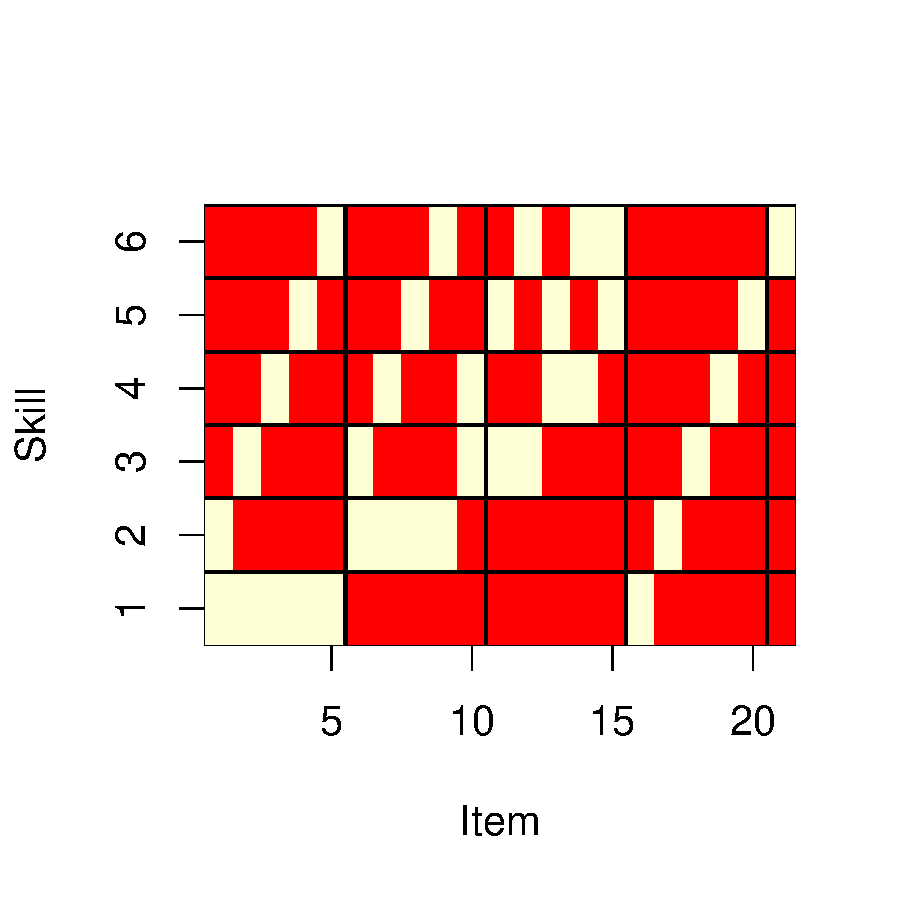
\includegraphics[scale =0.5] {ExpectedQ.pdf}\label{PerfectQ1}
 }\quad
 \subfigure[Synthetic data of 100 students with 10\% slip and 20\% guess factor]{
   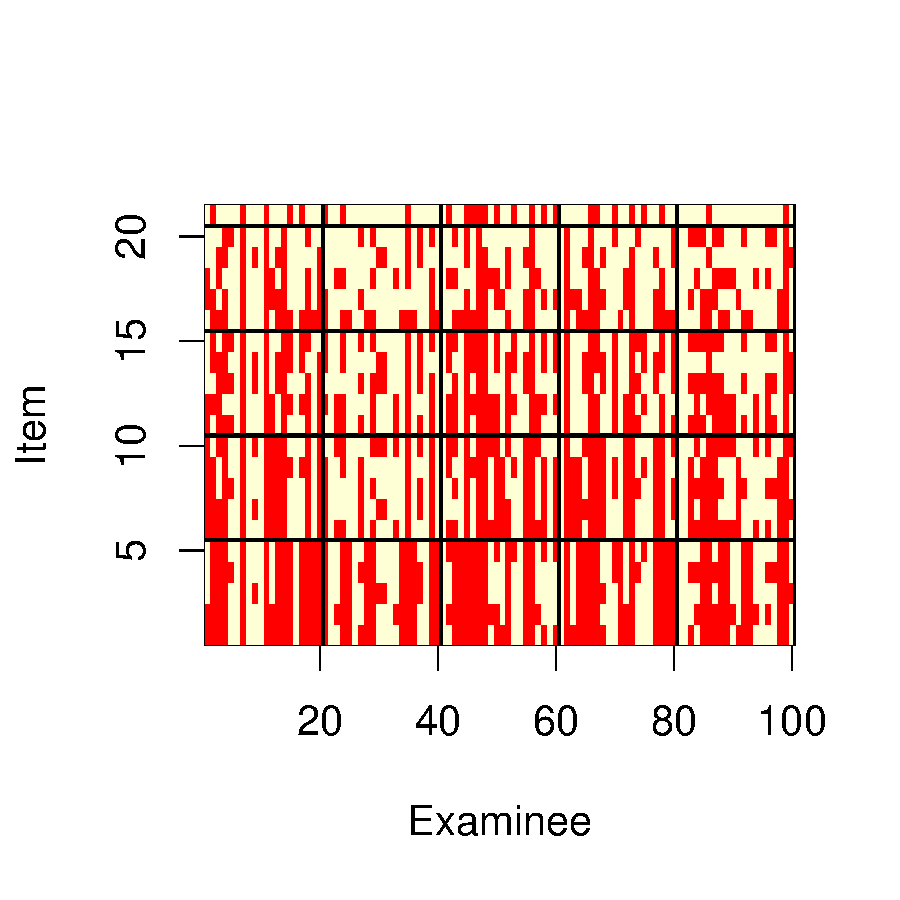
\includegraphics[scale =0.5] {ResultM.pdf}\label{Result_ofPerfectQ}
 }
\caption{Q-matrix and an example of simulated data with this matrix.  pale cells represent 1's and red ones represent 0's.}
\label{figqmatrixandResutM}
\end{figure}



\subsection{Noise factor}
\label{Noise_}
Finally, two more parameters are used in the simulated the data, namely the $\mathit{slip}$ and $\mathit{guess}$ factors. They are essentially noise factors and there are three approaches to apply these factors to the result matrix:
\begin{itemize}
\item Student based: each student would have specific amount of these factors in his test result.
\item Item based: this represent how tricky a question can be. The greater they are, the more tricky is the task of inducing the Q-matrix from data. This approach is used in DINA/DINO models.
\item Overall: for linear models of data generation we use this type of noise. For example, with $s\%$ of slip and $g\%$ of guess factor ,this will result in approximately $s\%$ of the succeeded items to become failed, and $g\%$ of the failed items to become succeeded in the test outcome matrix.

\end{itemize}

A sample of the results matrix for conjunctive model and additive model is given in figure~\ref{Result_ofPerfectQ} and  \ref{NMFAddNoisy} respectively where pale cells represent a value of 1 and red cells are 0. Examinee ability shows up as vertical patterns, whereas skills difficulty creates horizontal patterns. As expected, the mean success rate of the 2-skills items 1 to 15 is lower than the single skill items 16 to 21. The same situation for additive model in figure \ref{figNMFAddgen} , for additive models in figure  \ref{NMFAddNonNoisy} the patterns are more tangible where there are shades of colors that indicate different probability of success. Once the result matrix is created we need to discretize the values with respect to average success rate. Figure \ref{NMFAddNoisy} shows a Discretized version of result matrix with 20\% slip and 10\% guess factor.

 \begin{figure}[ht]
\begin{tabular}{c}
\subfigure[{Additive Q-matrix\label{figNMFAddQM}}]{\begin{footnotesize}
$\begin{array}{ccc}
 && \textrm{items}\\

\mathrm{\begin{sideways}skills\end{sideways}} & & \left[\begin{array}{cccccccccccccccccc}

0.00&0.00&0.25&0.00&0.00&0.00&0.33&0.33&0.5&0.0&0.0&0.5&0.0&0&0&0&0\\
0.25&0.00&0.25&0.25&0.00&0.00&0.00&0.33&0.0&0.0&0.0&0.0&0.0&0&1&0&0\\
0.25&0.25&0.25&0.25&0.00&0.33&0.00&0.33&0.0&0.5&0.0&0.0&0.0&1&0&0&0\\
0.25&0.25&0.00&0.00&0.33&0.33&0.00&0.00&0.5&0.0&0.5&0.0&0.0&0&0&0&0\\
0.25&0.25&0.00&0.25&0.33&0.33&0.33&0.00&0.0&0.0&0.0&0.0&0.5&0&0&1&0\\
0.00&0.25&0.25&0.25&0.33&0.00&0.33&0.00&0.0&0.5&0.5&0.5&0.5&0&0&0&1


\end{array}\right]
\end{array}$
\end{footnotesize}
}\\
\begin{tabular}{cc}
\subfigure[Raw Result matrix ]{
   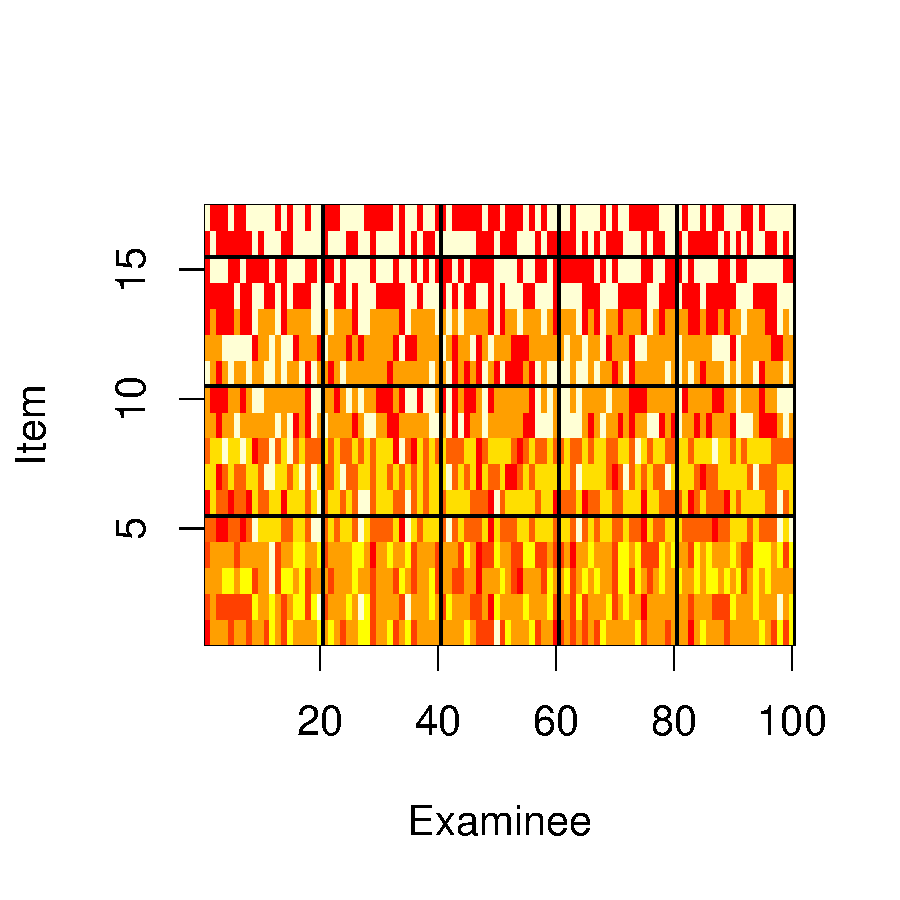
\includegraphics[scale =0.5] {NMFAddNonNoisy.pdf}\label{NMFAddNonNoisy}
 }\quad
&
\subfigure[Discretized result matrix with 20\% slip and 10\% guess factor]{
   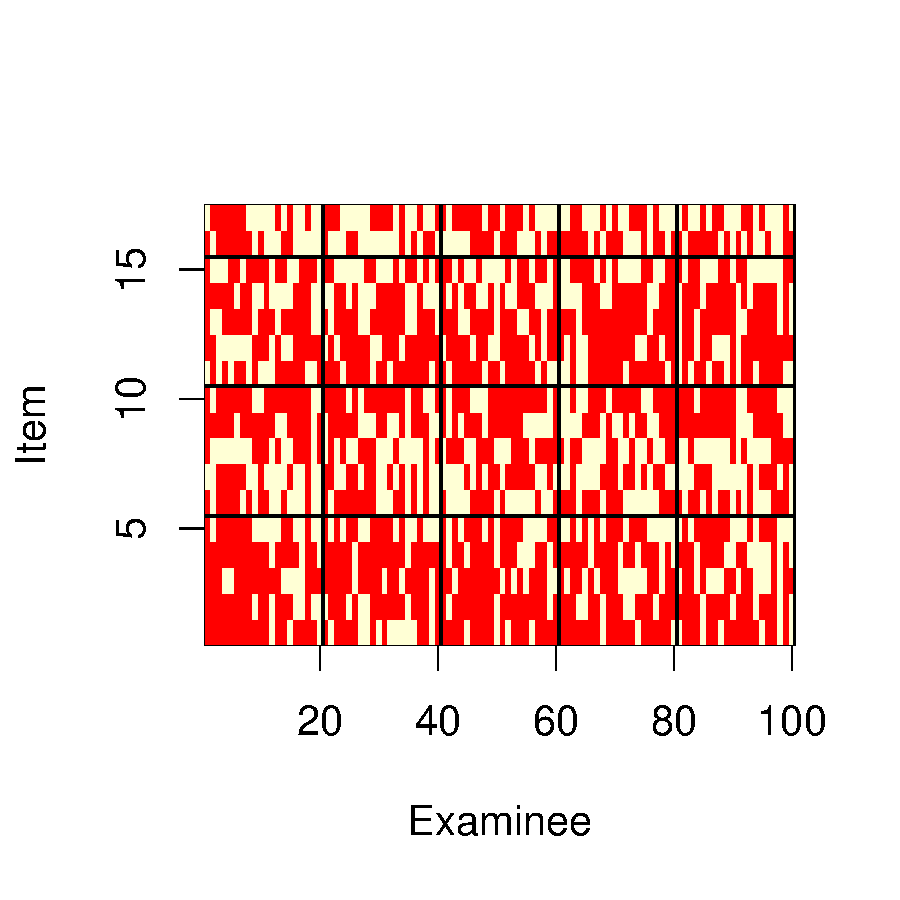
\includegraphics[scale =0.5] {NMFAddNoisy}\label{NMFAddNoisy}
 }\quad
\end{tabular}
\end{tabular}
\caption{Additive model of Q-matrix and Corresponding synthetic data}
\label{figNMFAddgen}
\end{figure}




%There are two ways to apply item variance in the simulated data and both of them are based on manipulating the values of the Q-matrix. Applying skills difficulty on skills would transfer the difficulty to items that have this skill. The other method is to consider the same weight for skills difficulty but controlling the item variance by assigning different number of skills to items. For example items with 1 skill would become easier to answer comparing to items with two or more skills where skills difficulty is the same for all skills. 

%The second step is to create a student skills mastery matrix which maps $k$ skills to $m$ students. In terms of ability for examinees we assigned random values to skills for students but  student variance show up as the variance in number of skills across examinees. At the same time we can apply the overall success rate on the skill mastery matrix using a threshold to discrete the assigned values in skills mastery. 

%Once the Q-matrix and Skills mastery matrix is created we can produce the test result matrix with equation~(\ref{eq:6}). The last step is to add slip and guess factors which are set as constant values across items.



%\section{Linear NMF Additive}





\section{Cognitive Diagnosis Models}

From the family of cognitive diagnosis models we choose two models which are deterministic input noisy AND/OR. Detailed description of these models is given in section \ref{DINA-DINO-Desc}. This section discusses the approach that we took to generate synthetic datasets based on these models. The same as linear models, these models also represent the mapping of multiple skills to items and examinees in a form of a Q-matrix and skills mastery matrix respectively. To borrow the Q-matrix form an existing dataset we use NMF because these models can not infer a Q-matrix but they can estimate other model specific parameters such as student profile, slip and guess given a Q-matrix. 

%These models are also categorized as linear models that use a Q-matrix. The Q-matrix can be predefined for a better comparison or can be synthetic. For synthetic Q-matrix we use the same method as described before. At the same time we can control the number of skills and items in generation of a Q-matrix.

To obtain a conjunctive type of Q-matrix for DINA model we follow the same approach as described in section \ref{Q-MatrixObtain} where the normalization process does not apply.  Generating the student profile is almost the same as section \ref{Student_Profile} but there are other parameters involved:

% Examinee's skills can be generated by a normal distribution which should match the number of skills presented in the Q-matrix. The difference between creation of skills mastery matrix in DINA/DINO and NMF is the way that skills are appearing for each student. In DINA/DINO there is a predefined set of possible combination of skills that can be used in skills mastery for each student. For example for 3 skills, this set can have maximum 8 combination. There is a distribution that is assigned to this set which defines the probability of appearance for each combination in the skills mastery matrix. 
 
\subsection{Skill space}
Assuming $K$ skills, there are possibility of $2^K$ combination of skills to be assigned to student profile. This shows the maximum capacity of skill space. One of the parameters of student profile is skill class where only few candidate in the space of skills combination are allowed for skills mastery matrix. This parameter has a benefit that can control the prerequisite skill in a student skills mastery vector given a partial order structure of skills.

\subsection{Skill distribution}

There is a distribution that is assigned to skill class set which defines the probability of appearance for each combination indicated in skills class. i.e. If there exists 3 skills then the skill space will be 8 combinations and assuming skill class have 4 combinations out of these 8, then skill distribution  must be a vector of length 4, with sum equal to 1. With this parameter student score variance can be manipulated. We use a normal distribution in this research to assign skills to examinees.



\begin{center}
$Student$  $skills \sim \pN(\mu, s_s)$
\end{center}

With these two parameters a skill mastery matrix can be generated randomly.

\subsection{Slip and Guess}
These parameters are essentially noise factors and in these models they are treated item wised (section \ref{Noise_}). We defined a uniform distribution to cover a range of values for slip and guess:


\begin{center}
$Slip \sim \textit{U}(S_{lower-bound}, S_{upper-bound})$

$Guess \sim \textit{U}(G_{lower-bound}, G_{upper-bound})$
\end{center}

Once all the parameters are prepared we can generate an outcome of test $j$ for examinee $i$ from equation~\ref{DinoEQ3} where $\xi_{ij}$ is calculated based on AND or OR gates. Since these models are behaving based on a single value that represents student ability, we need to calculate an array of abilities for each item given a set of skills for an student. For DINO a disjunction is used between skills of an item and skills of a student to determine whether the student has the ability or not where for DINA a conjunction applies.

\begin{equation}
 R_{ij} \,=\, (1-s_j)^{\xi_{ij}} g_j^{1-\xi_{ij}}
\label{DinoEQ3}
\end{equation}

\section{Educational data generator}

Despite all the parameters and models that were described, it is still challenging to generate synthetic data for a specific model with a set of given parameters. We \citep{Trieu2015} created a package that generates synthetic data under a specific model's assumption given a set of parameters. As mentioned before these parameters can be fine grained which can be combined to create a more complex parameter. In this sense we can create a hierarchy for the complexity of these parameters. 

Previous sections described the generation process for each model. This task is easy and possible as long as two conditions are satisfied: 
\begin{itemize}
\item First: All the parameters for a model are given. Table \ref{tbl:param-DataGen} shows a list of required parameters to generate synthetic data.
\item Second: There exists no conflict between the given parameters. For example given ``number of skills'' as a simple parameter equal to $4$ and a predefined ``Q-matrix'' as a complex one with $5$ skills is a conflict to generate a synthetic data based on DINO model. However, testing these conflicts is not an easy task and also resolving a conflict is another challenge.
\end{itemize} 

For some of parameters we can use default values but some are mandatory such as number of skills. Therefore based on the hierarchical structure among parameters of a model we can define sets of sufficient parameters to generate data based on a model. Due to this structure there are different combination of parameters that can generate a synthetic data. For example, a synthetic dataset based on DINA can be generated with {Q-matrix, Skills mastery matrix, Slip and Guess vectors} or {Number of skills, Items and students}. Figure \ref{Line_Conj_Pars} shows the hierarchical structure of the required parameters for linear conjunctive model. This graph can be extended to other models. 

\begin{figure}[ht]
\centering
 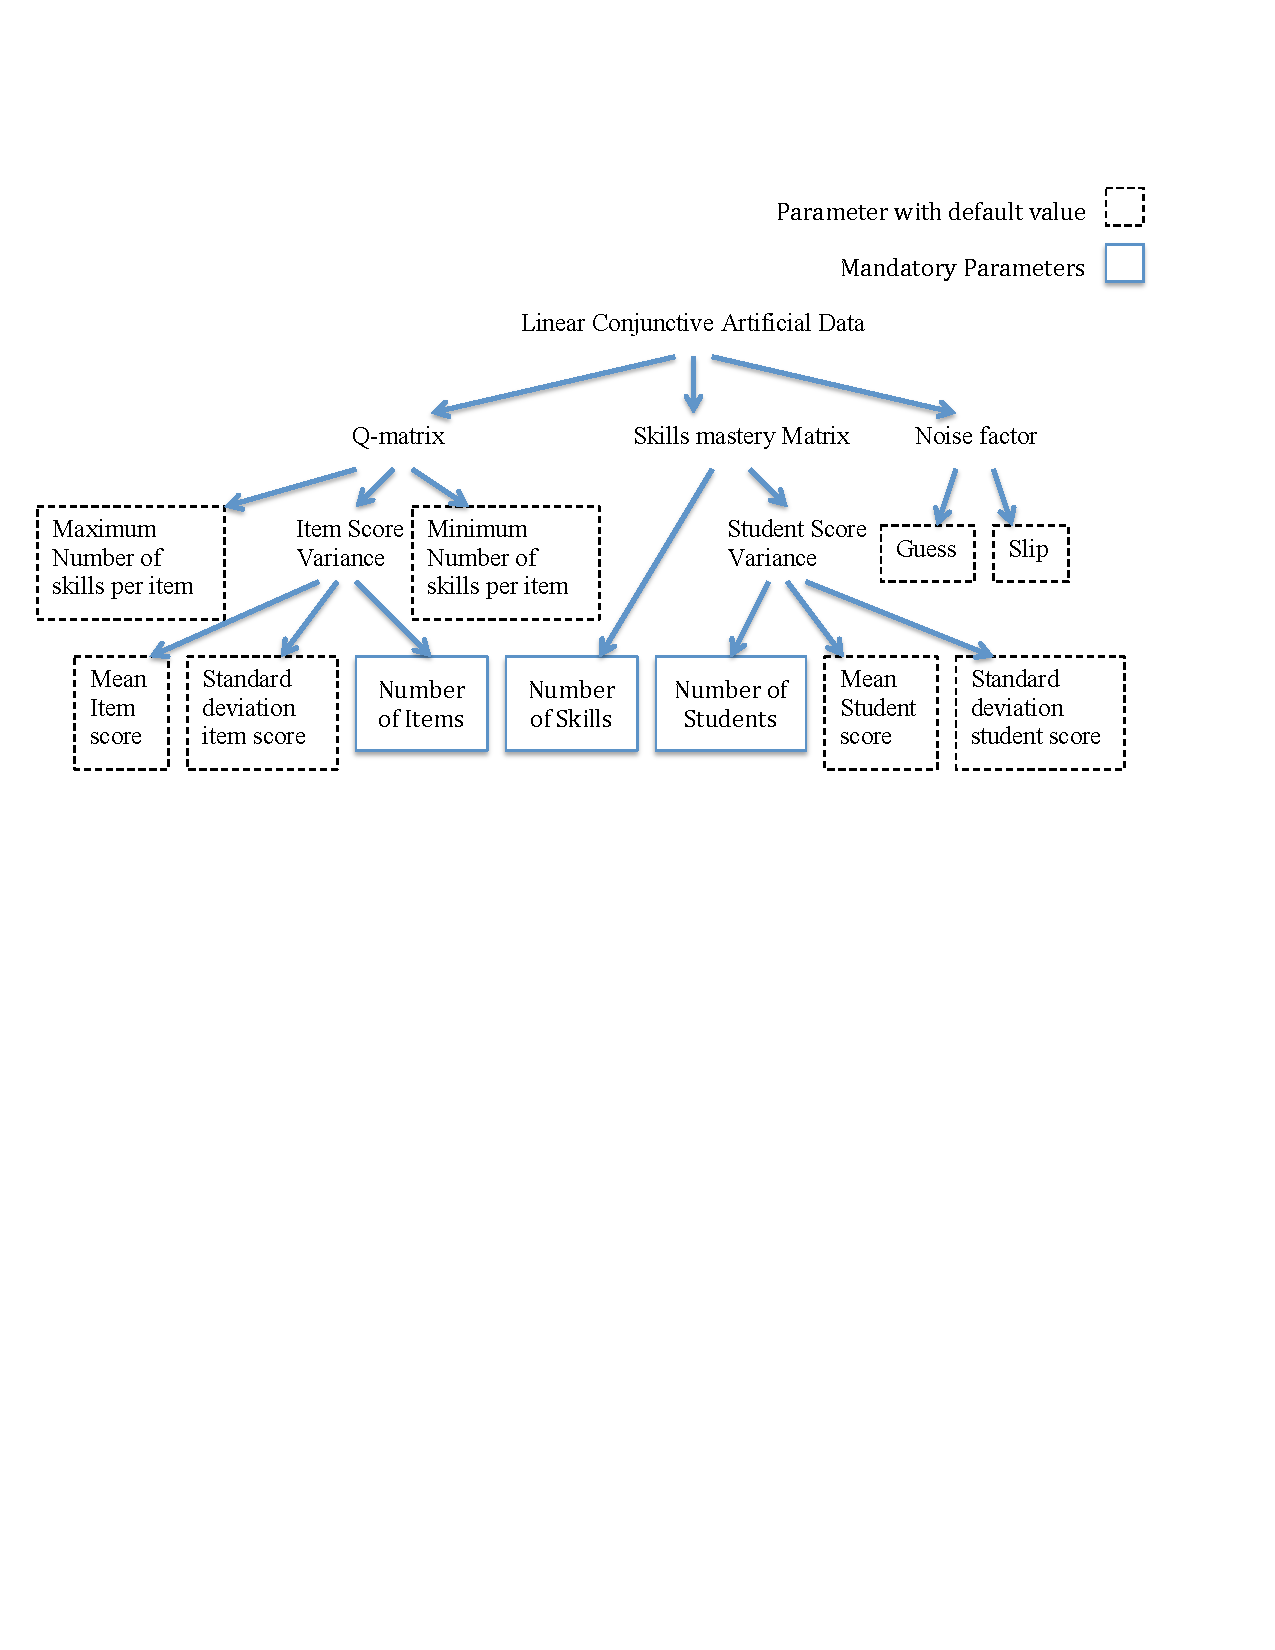
\includegraphics[trim= 3cm 15cm 5cm 3cm, scale =0.85] {Linear_Conj_Pars.pdf}\label{PerfectQ}
\caption{hierarchical structure of parameters of linear conjunctive model}
\label{Line_Conj_Pars}
\end{figure}

There exist some intermediate steps between the lower level(simple) and higher level(more complex) parameters which can potentially result in a variance in the generated data. The goal of creating this package is to efficiently use the available parameters to generate data based on different models where potential conflicts and exceptions are covered. 

%The global variable ``Context'' in this package is capable to save upto 62 parameters which are required by all models. 


%R package edmsyn provides users a simple framework that conveniently handles all the situations above while generating data, including checking for condition 1 and condition 2. It also automates the process of learning parameters from raw data, modifying and using this information to create synthetic data from 10 different models. This document is intended to give a quick and thorough tutorial on using edmsyn.


%Since some of the parameters are shared between different models, edmsyn did not regard the collection of all parameters from 10 models separately, but jointly as different aspects describing a single instance of reality. For example, the vector of discrimination factors of all items is a parameter belongs to the IRT-2pl model, which is not the case for the parameter Q-matrix, however, edmsyn introduces the class context where these two parameters co-exist in a single object and can be utilized according to user purpose.

